\documentclass[12pt, a4paper]{report}
\usepackage[utf8]{inputenc}
\usepackage[a4paper, portrait, margin=1in]{geometry}
\usepackage{listings}
\usepackage{color}
\usepackage{graphicx}

\definecolor{codegreen}{rgb}{0,0.6,0}
\definecolor{codegray}{rgb}{0.5,0.5,0.5}
\definecolor{codepurple}{rgb}{0.58,0,0.82}
\definecolor{backcolour}{rgb}{0.95,0.95,0.92}

\lstdefinestyle{mystyle}{
    backgroundcolor=\color{backcolour},
    commentstyle=\color{codegreen},
    keywordstyle=\color{magenta},
    numberstyle=\tiny\color{codegray},
    stringstyle=\color{codepurple},
    basicstyle=\footnotesize,
    breakatwhitespace=false,
    breaklines=true,
    captionpos=b,
    keepspaces=true,
    numbers=left,
    numbersep=5pt,
    showspaces=false,
    showstringspaces=false,
    showtabs=false,
    tabsize=2
}

\lstset{style=mystyle}


\title{Network application to acquire data from multiple GCO connections and
	   transmit combined data as a single GCO link to TDACS}
\author{Sai Charla}
\date{\today}


\begin{document}
\maketitle
\tableofcontents


\chapter*{Abstract}
\addcontentsline{toc}{chapter}{\numberline{}Abstract}
\par This project is for developing an application to handle multiple satellite
Thermovac tests at once using a single TDACS system. No changes(Hardware and
software) in the existing system will be necessary. The application will be
loaded into a PC connected to both TDACS and Checkout networks.


\chapter{Introduction}

\par The current TDACS system is capable of handling data from a single
Checkout team and by extension only from one satellite. This makes simultaneous
Thermo-vac testing of multiple satellites cumbersome and error prone. In order
to overcome that bottleneck a network-merge application is designed which can
trick TDACS to process and store multiple satellite data as a single satellite
data. The user should have necessary naming conventions to differentiate the
data from different satellite. The scope of the current project is listed below:

	\begin{enumerate}
			\item Acquire GCO Data from multiple IP addresses(Multiple Satellites
					-Multiple Checkout teams).
			\item Processes the acquired data in to a single stream with the same
					protocols as received data.
			\item Send the data stream to TDACS system.
			\item This ensures the that no hardware or software changes are required
					for present system for acquiring multiple satellite data other than an
					additional PC which acquires data and relays the processed data as if it
					is received from one one GCO.
			\item An Application which can simulate all the above phenomena for
					testing.
	\end{enumerate}


\chapter{Application architecture}
The System acts as server to the present TDACS(which treats it as GCO itself)
and as an independent client to each and every GCO system (Satellite GCO).

\begin{figure}[!h]
	\centering
	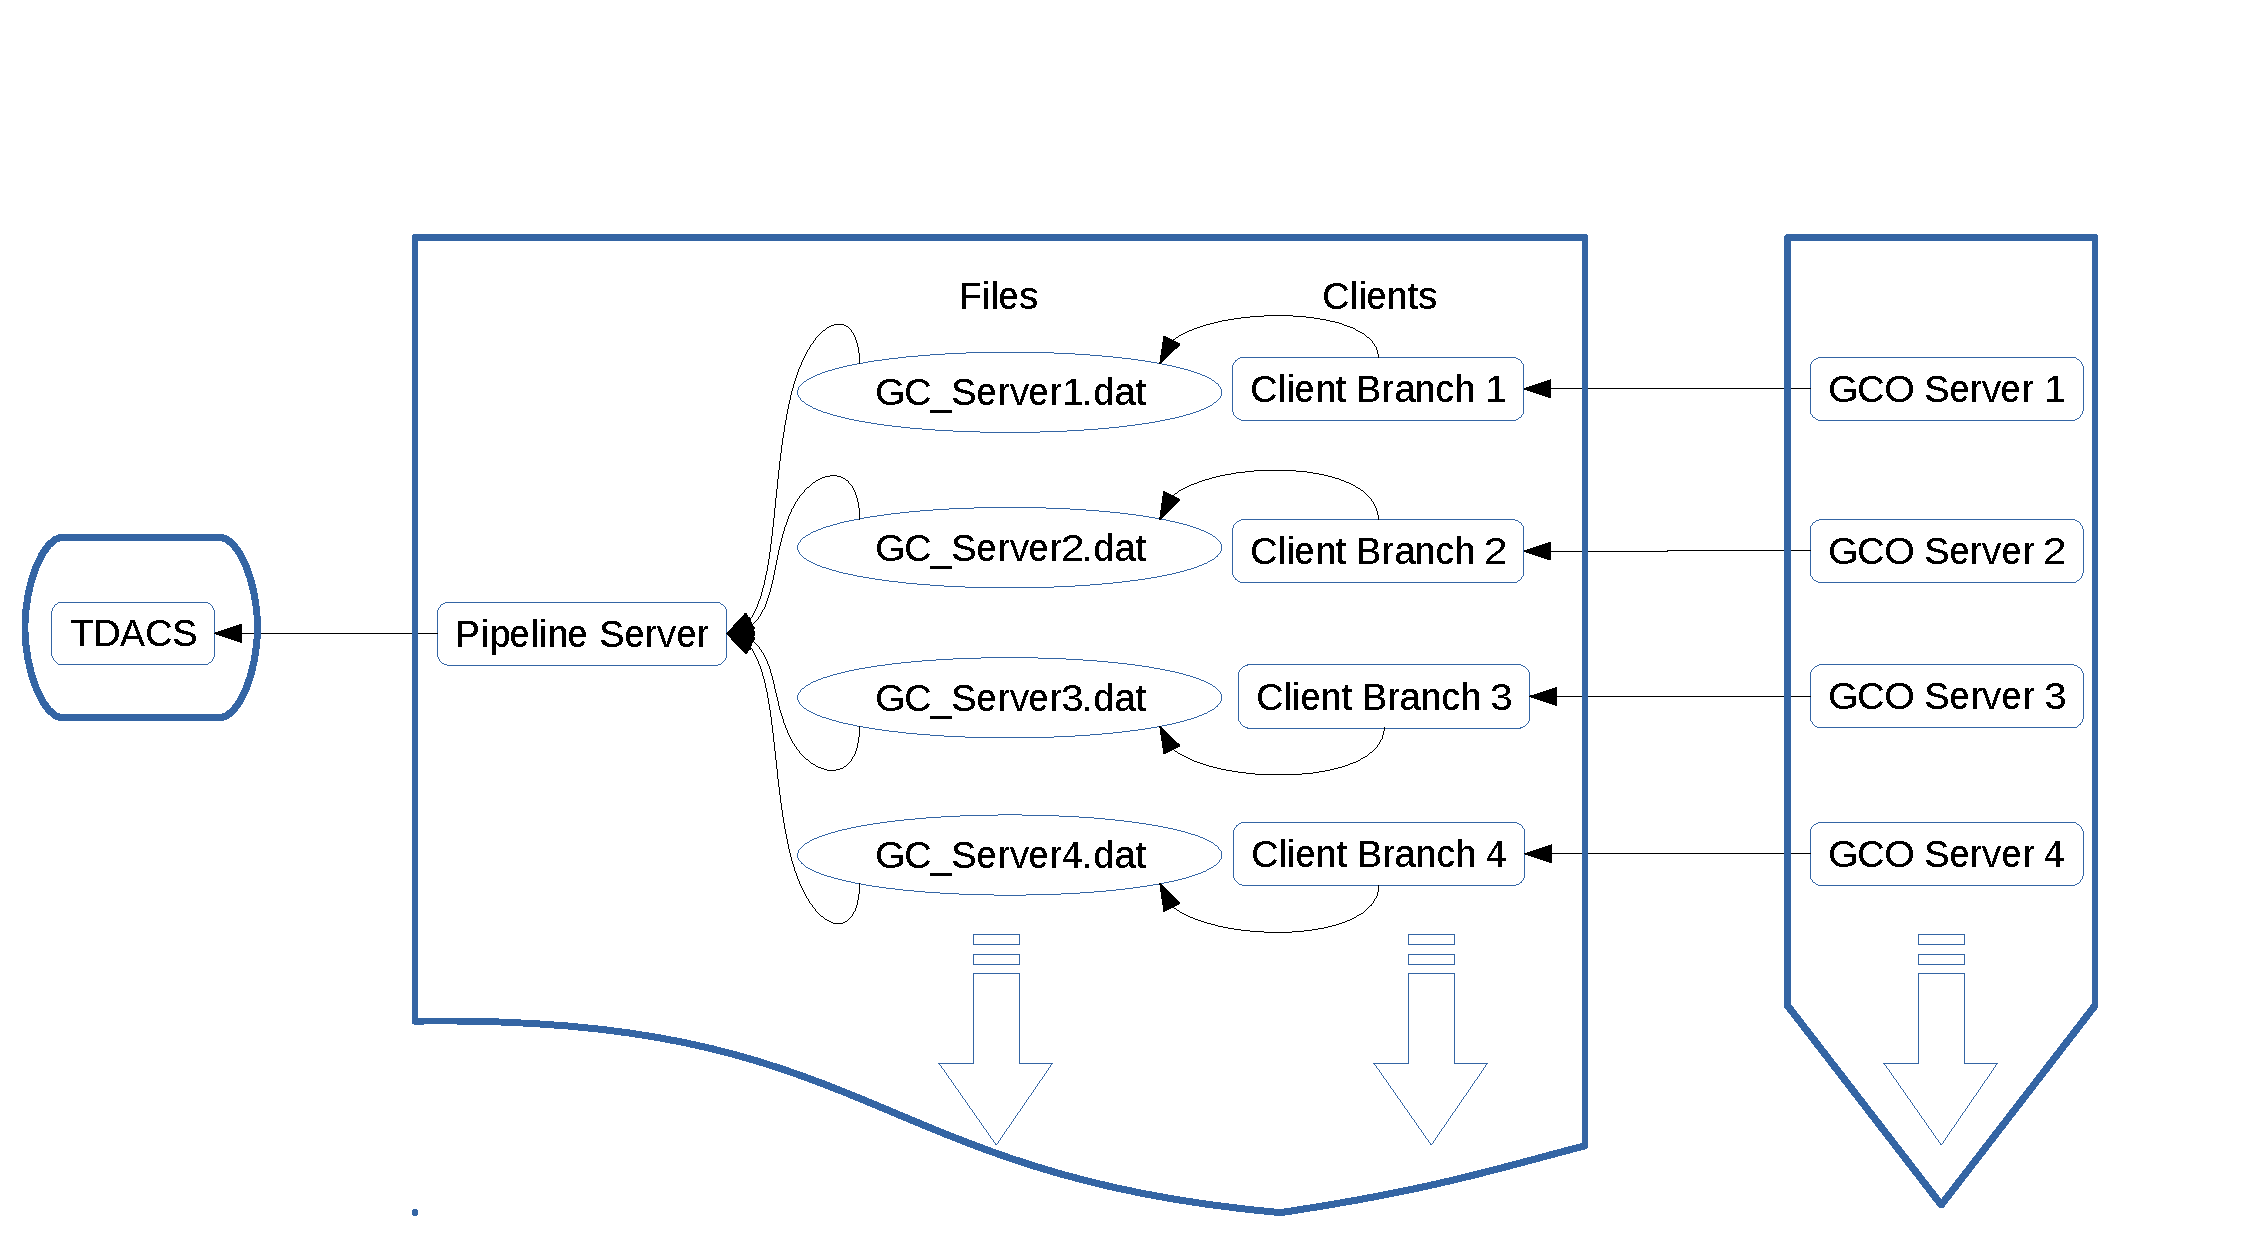
\includegraphics[scale=0.4]{arch.pdf}
	\caption{Architecture of the application}
\end{figure}

\par The above figure shows how the application handles multiple satellite data
and how it connects to the TDACS and also the Ground Checkout Systems. The
application spawns off a client branch for every ground checkout server and
writes the data in to a .dat file named after the server's address(HOST\_PORT).
Then the Pipeline Server sequentially reads each of those files concatenates
the data and sends it to the TDACS.

\chapter{Source Code Documentation}
The main source code spreads across the following python files namely:
\begin{enumerate}
	\item pipeline\_server.py
	\item client\_branch.py
	\item protocol.py
	\item fileilockio.py
	\item config.py
\end{enumerate}
The confuguration of the application is set using 2 configuration files namely:
\begin{enumerate}
	\item GC.conf
	\item pipeline.conf
\end{enumerate}

\section{Configuration Files}

\subsection{GC.conf}
This file will contain the necessary details of the Ground Checkout servers
including hostname, port, no. of parameters and the sampling time. An example
of GC.conf is shown as below:
\lstinputlisting{../GC.conf}

\subsection{pipeline.conf}
This file contains the details required for setting up the pipeline server
including hostname, port and the sampling time. An example of pipeline.conf is
shown below:
\lstinputlisting{../pipeline.conf}


\section{Python Modules}

\subsection{config.py}
This file has 2 functions namely $get\_config()$ and $pipeline\_config()$ which
parse GC.conf and pipeline.conf respectively an return the configuration
details in proper object type and format.
%\begin{itemize}
%	\item get\_config([GC.conf]) $->$ int n, (str, int)\_array addrs, int\_array nparms,
%		int\_array st\_list
%	\item pipeline\_config([pipeline.conf]) $->$ (str, int)\_array addrs, int\_array
%		sleeptime
%\end{itemize}


\subsection{filelockio.py}
This file has 2 functions namely $filelockread()$ and $filelockwrite()$ which read
and write in to files with a lock in place while reading or writing to avoid
simultaneous reading and writhing by different processes.


\subsection{protocol.py}
This file contains the functions and classes for creating and manipulating the
Ground Checkout data frames. The various contents of the file are listed below:


\subsection{pipeline\_server}
This file contains the PipelineServer class which creates a PipelineServer
object which connects to



\chapter{Future Scope}
\par The following augmentations to the current project are suggested:
\begin{enumerate}
	\item Include a database which stores the incoming data by reading the
		files at specified intervals of time. An SQLite3 database would be
		ideal.
	\item Include real-time plotting feature on to the database using Pandas
		and Matplotlib.
	\item Augment the protocol to get more satellite data and store it in the
		database while sending only part of it which is in accordance with the
		TDACS protocol.
\end{enumerate}


\chapter*{References}
\addcontentsline{toc}{chapter}{\numberline{}References}
	\begin{itemize}
			\item Learning Python Network Programming- Dr.M.O. Faruque Sarkar, Sam
					Washington.
			\item The Definitive Guide to Linux Network Programming- Keir Davis, John
					W.Turner and Nathan Yocom.
			\item Internetworking With TCP/IP vol-III, Client-Server Programming and
					Applications (BSD Socket Version)-David L. Stevens, Douglas E. comer
			\item www.python.org
	\end{itemize}

\appendix
\chapter*{Appendix A: Instructions for running the program}
\addcontentsline{toc}{chapter}{\numberline{}Appendix A: Instructions for
running the program}
\begin{enumerate}
	\item Update the GC.conf file with the host names, ports, number of
		parameters and sampling times of each ground checkout servers in a new
		line (Number of non-comented lines will be counted for finding the total
		number of ground checkout servers). Make sure that the system is able to
		ping to each of those hosts.
	\item Update the pipeline.conf with the host name, port and samplng time.
		Make sure that the system is able to ping to TDACS.
	\item Run the file pipeline\_server.py. In terminal type:
		$$python \quad pipeline\_server.py$$
	\item Check the status of the application regularly.
\end{enumerate}




\chapter*{Appendix B: Ground Checkout communication protocol}
\addcontentsline{toc}{chapter}{\numberline{}Appendix B: Ground Checkout communication protocol}
\par The communication protocol between Ground Checkout and TDACS is text based
over TCP/IP. The frame in encoded using \textbf{ASCII} character code set.
There are 2 types of data packets namely:

\begin{enumerate}
	\item Data Frame
	\item Data Base Frame
\end{enumerate}
A sample of varius data frames are shown as follows:
\lstinputlisting{gc_data.txt}
\newpage
If F is a Ground checkout frame, the varius elements of the ground checkout
frame are listed as below:

% Frame details (Afterf stripping STX and ETX):
% frame[0] = frame type (DATA, DB)
% frame[1:18] = time stamp
% frame[18:22] = no. of parms
% frame[22:27] = white spaces
% frame[27:] = data
% if DATA: len = 8 bytes
% if DB: len = 25 bytes

\begin{itemize}
	\item F[0] : ASCII Start of Text (STX) : '0x02'
	\item F[1] : Byte designating the type of frame : '0xcc' - Data Base Frame,
		'0xbb' - Data Frame
	\item F[2:19] : Time stamp of the frame :  DDMMYYYYhhmmss000 (the trailing
		zeros are for milliseconds if used)
	\item F[19:23] : Number of parameters in the frame
	\item F[23:28] : Mandatory White Spaces
	\item F[28:-1] : Data : 8 bytes for each parametes if it is a Data Frame
		and 25 bytes for each parameter if it is Data Base Frame.
		\begin{itemize}
			\item For 8 bytes of parameter value in Data Frame:
				\begin{itemize}
					\item bytes[0] : Sign of the value $\pm$
					\item bytes[1:8] : Floating point value rounded to 2
						digits after decimal.
				\end{itemize}
			\item For 25 bytes of Parameter name in Data Base Frame:
				\begin{itemize}
					\item bytes[0:4] : PID number
					\item bytes[4:19] : Mnemonic for the parameter
					\item bytes[19:24] : Unit
					\item bytes[24] : Analog - 1 or Digital - 2
				\end{itemize}
		\end{itemize}
	\item F[-1] : ASCII End of Text (ETX) : '0x03'
\end{itemize}
\bigskip
The parameters with truth values like On/Off, Enable/Disable, BothEnamble/..
etc., are sent as text in those 8 bytes padded with necessary number of spaces
at the end. These are mapped to $1/0$ in the datbase of TDACS and stored. Other
values are converted in to floating point numbers and stored.



\end{document}
